\chapter{Confidence Intervals}

\section{Definition}

So far, we have seen how we can estimate an unknown population parameter from a random sample. For instance, if the parameter we seek to estimate is the mean $\m$, we can employ an unbiased estimator, i.e. the sample mean $\ol{x}$, to get a rough value for $\m$. This is what we call a \vocab{point estimate}. However, a point estimate does not provide any information about the uncertainty present. To this end, it is more desirable to obtain an interval estimate.

\begin{definition}
    An \vocab{interval estimate} of an unknown population parameter is a random interval constructed so that it has a given probability of including the parameter.
\end{definition}

This leads us to the notion of a confidence interval.

\begin{definition}
    Given a fixed value $\a \in [0, 1]$ (known as the \vocab{level of significance}), a \vocab{$100(1 - \a)$\% confidence interval} for an unknown population parameter $\t$ is any interval $(a, b)$ such that \[\P{a < \t < b} = 1 - \a.\]
\end{definition}

As an example, let us take $\a = 0.05$. If we can find a method of calculating the limits $a$ and $b$, this means that in the long run, if we repeatedly take samples, then the calculated interval $(a, b)$ will contain the population parameter $\t$ for 95\% of the samples taken. Equivalently, the probability of obtaining a random sample for which the corresponding interval contains $\t$ is $0.95$.

Note however, that for a particular sample, we do not know whether this is one of the samples for which $\t$ is in the sample. Our ``confidence'' in the interval comes from the fact that we are using a formula which gives a correct result \emph{most of the time}.

We can express the above notions diagrammatically:

\begin{figure}[H]
    \centering
    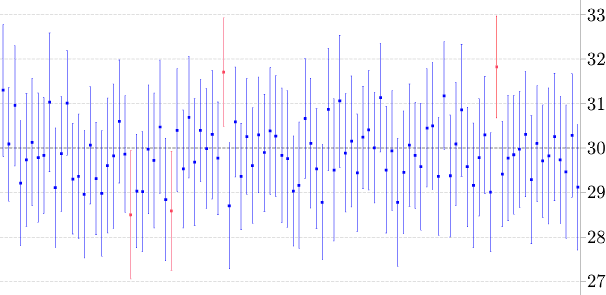
\includegraphics[scale=0.5]{media/confidence interval.png}
    \caption{One hundred 95\% confidence intervals for $\m$ ($= 30$) computed from 100 different samples. Confidence intervals coloured red do not contain $\m$.\protect\footnotemark}
\end{figure}
\footnotetext{Source: \url{https://amsi.org.au/ESA_Senior_Years/SeniorTopic4/4h/4h_2content_10.html}}

\section{Population Mean}\label{S:Confidence-Intervals-Mean}

In this section, we explore interval estimates for the population mean $\m$.

Recall that for a significance level of $\a$, we wish to find an interval $(a, b)$ such that \[\P{a < \m < b} = 1 - \a.\] To make our lives easier, we impose the restriction that the confidence interval be symmetric about $\m$, that is, the interval should be of the form $(\m - E, \m + E)$, where $E$ is the \vocab{margin of error}. However, we obviously do not know $\m$, so we make use of the next best thing available: $\ol{x}$, to get something of the form \[\bp{\ol{x} - E, \, \ol{x} + E}.\] We thus wish to find the value of $E$ such that
\begin{equation}\label{eqn:CI}
    \P{\ol{x} - E < \m < \ol{x} + E} = 1 - \a.
\end{equation}
Depending on the situation, $\m$ will be distributed differently, so $E$ will differ accordingly.

There are four cases we will consider, with their respectively subsection numbers labelled in the table below:

\begin{table}[H]
    \centering
    \begin{tabular}{|c|c|cc|}
    \hline
    \multirow{2}{*}{$\s^2$} & \multirow{2}{*}{$n$} & \multicolumn{2}{c|}{Population Distribution} \\ \cline{3-4} 
    &  & \multicolumn{1}{c|}{Normal} & Unknown \\ \hline
    \multirow{2}{*}{Known} & Large & \multicolumn{1}{c|}{\multirow{2}{*}{\SS\ref{S::CI:1}}} & \SS\ref{S::CI:2} \\ \cline{2-2} \cline{4-4} 
    & Small & \multicolumn{1}{c|}{} & \cellcolor{black} \\ \hline
    \multirow{2}{*}{Unknown} & Large & \multicolumn{2}{c|}{\SS\ref{S::CI:3}} \\ \cline{2-4} 
    & Small & \multicolumn{1}{c|}{\SS\ref{S::CI:4}} & \cellcolor{black} \\ \hline
    \end{tabular}
\end{table}

\subsection{Normally Distributed Population with Known Variance}\label{S::CI:1}

Suppose our population is normally distributed with unknown mean $\m$ and known variance $\s^2$, so $X \sim \Normal{\m}{\s^2}$. In the previous chapter, we learnt that \[\ol{X} \sim \Normal{\m}{\frac{\s^2}{n}},\] where $n$ is the sample size. If we standardize this, we get \[Z = \frac{\ol{X} - \m}{\s / \sqrt{n}},\] where $Z$ is the standard normal distribution $\Normal{0}{1}$. Manipulating (\ref{eqn:CI}), we get \[\P{\ol{x} - E < \m < \ol{x} + E} = \P{-\frac{E}{\s/\sqrt{n}} < \frac{\ol{x} - \m}{\s/\sqrt{n}} < \frac{E}{\s/\sqrt{n}}} = 1 - \a.\] But we recognize the middle expression as $Z$, so we really have \[\P{-\frac{E}{\s/\sqrt{n}} < Z < \frac{E}{\s/\sqrt{n}}} = 1 - \a.\] Because $Z$ is symmetric about 0, we can finally isolate $E$: \[\P{0 < Z < \frac{E}{\s/\sqrt{n}}} = \frac{1-\a}{2} \implies \P{Z < \frac{E}{\s/\sqrt{n}}} = 1 - \frac{\a}{2}.\] We now introduce some notation regarding $z$-values.

\begin{definition}
    Given a probability $c \in [0, 1]$, the \vocab{critical value} $z_c$ is defined as \[\P{Z < z_c} = c,\] i.e. it acts as an ``inverse'' to the standard normal distribution.
\end{definition}

With this notation, we can isolate our margin of error $E$: \[\frac{E}{\s/\sqrt{n}} = z_{1 - \frac\a2} \implies E = z_{1 - \frac\a2} \frac{\s}{\sqrt{n}}.\] We thus obtain the following result:

\begin{proposition}
    If $X$ is normally distributed and has known variance $\s^2$, then the symmetric $100(1-\a)$\% confidence interval for $\m$ is given by \[\bp{\ol{x} - z_{1 - \frac\a2} \frac{\s}{\sqrt{n}}, \, \ol{x} + z_{1 - \frac\a2} \frac{\s}{\sqrt{n}}}.\]
\end{proposition}

The two limiting values that define the interval are known as the \vocab{$100(1-\a)$\% lower and upper confidence limits}, sometimes writen as \[\ol{x} \pm z_{1 - \frac\a2} \frac{\s}{\sqrt{n}}.\]

Graphically, the area under $\Normal{\ol{x}}{\s^2}$ over the confidence interval is $1 - \a$:

\begin{figure}[H]\tikzsetnextfilename{475}
    \centering
    \begin{tikzpicture}[trim axis left, trim axis right]
        \begin{axis}[
            domain = 0.5:3.5,
            xmin = 0.5,
            xmax = 3.5,
            ymax = 1,
            ymin = -0.1,
            restrict y to domain =-10:5,
            samples = 101,
            axis x line=middle,
            xtick = {2, 1.168, 2.832},
            xticklabels = {$2$, $2 - z_{0.975} \frac{3}{\sqrt{50}}$, $2 + z_{0.975} \frac{3}{\sqrt{50}}$},
            y axis line style={opacity=0},
            ytick=\empty,
            legend cell align={left},
            legend pos=outer north east,
            ]
            
            \addplot[fill=orange!20, draw=none, domain=1.168:2.832] {gauss(2,0.4243)} \closedcycle;
            \addplot[black, very thick] {gauss(2, 0.4243)};
            \draw[dashed] (2, 0) -- (2, 0.940);
        \end{axis}
    \end{tikzpicture}
    \caption{An illustration of a 95\% confidence interval for $\ol{x} = 2$, $\s = 3$ and $n = 50$.}
\end{figure}

\begin{sample}
    After a rainy night, 12 worms surfaced on the lawn. Their lengths, measured in cm, were: \[9.5, \, 9.5, \, 11.2, \, 10.6, \, 9.9, \, 11.1, \, 10.9, \, 9.8, \, 10.1, \, 10.2, \, 10.9, \, 11.0.\] Assuming that this sample came from a normal population with variance 4, calculate a 99\% confidence interval for the mean length of all worms in the garden.
\end{sample}
\begin{sampans}
    Let $X$ cm be the length of a worm. We have $\s = 2$ and $n = 12$. From the sample, we calculate $\ol{x} = 10.392$. Feeding this into the above expression, we see that a 99\% confidence interval for the mean length of all worms in the garden is \[\bp{10.392 - z_{0.995} \frac{2}{\sqrt{12}}, 10.392 + z_{0.995} \frac{2}{\sqrt{12}}} = (8.90, 11.9).\]
\end{sampans}

\subsection{Large Sample Size from Any Population with Known Variance}\label{S::CI:2}

In the case where the sample size is large ($n \geq 30$), we can invoke the Central Limit Theorem, regardless of the distribution of the population. If $X$ has variance $\s^2$, then we know from the previous chapter that \[\ol{X} \sim \Normal{\m}{\frac{\s^2}{n}} \text{ approximately}.\] By a similar argument as in \SS\ref{S::CI:1}, we obtain the following (more general) result:

\begin{proposition}
    If $X$ has known variance $\s^2$ and the sample size is large ($n \geq 30$), then the symmetric $100(1-\a)$\% confidence interval for $\m$ is given by \[\bp{\ol{x} - z_{1 - \frac\a2} \frac{\s}{\sqrt{n}}, \, \ol{x} + z_{1 - \frac\a2} \frac{\s}{\sqrt{n}}}.\]
\end{proposition}

\subsection{Large Sample Size from Any Population with Unknown Variance}\label{S::CI:3}

In most practical situations, it is likely that both the mean and variance are unknown. Provided that the sample size is large ($n \geq 30$), by the Central Limit Theorem, we can say that the distribution of $\ol{X}$ is approximately normal. In place of the unknown population variance $\s^2$, we use $s^2$, the unbiased estimate of the population variance as an approximation. Hence, \[\ol{X} \sim \Normal{\m}{\frac{s^2}{n}} \text{ approximately}.\] Just like before, we get the following result:

\begin{proposition}
    If $X$ has unknown variance but the sample size is large ($n \geq 30$), then the symmetric $100(1-\a)$\% confidence interval for $\m$ is given by \[\bp{\ol{x} - z_{1 - \frac\a2} \frac{s}{\sqrt{n}}, \, \ol{x} + z_{1 - \frac\a2} \frac{s}{\sqrt{n}}}.\]
\end{proposition}

\subsection{Normally Distributed Population with Unknown Variance and Small Sample Size}\label{S::CI:4}

Before looking at confidence intervals of $\m$ when the sample size is small, we first need to consider the Student's $t$-distribution.

\subsubsection{The $t$-distribution}

The crucial statistic in the construction of a confidence interval for the mean of a normal distribution is $Z$, given by \[Z = \frac{\ol{X} - \m}{\s/\sqrt{n}}.\] In \SS\ref{S::CI:3}, when $\s$ was unknown, we were able to $\s$ by $s$ by virtue of the large sample size, which allowed us to approximate $\ol{X}$ with a normal distribution.

In the present case, however, we do not have such a luxury. Now, when $\s$ is replaced by $S$, the random variable \[T = \frac{\ol{X} - \m}{S / \sqrt{n}}\] can no longer be apporixmated by a normal distribution. Here, $T$ depends on two random variables: namely $\ol{X}$ and $S$, the random variable corresponding to $s$. Note that the value of $T$ varies from sample to sample not only because of the variation in $\ol{X}$ as in the case of $Z$, but also because of the variation in $S$.

For samples of size $n$, it can be shown that \[T = \frac{\ol{X} - \m}{S / \sqrt{n}} \sim \StudentT{n - 1}.\] Note that this requires $X_1, \dots, X_n$ to have independent and identical normal distributions.

\begin{figure}[H]\tikzsetnextfilename{476}
    \centering
    \begin{tikzpicture}[trim axis left, trim axis right]
        \begin{axis}[
            domain=-2.5:2.5,
            samples=101,
            xmin = -2.5,
            xmax = 2.5,
            ymax = 0.45,
            ymin = -0.1,
            samples = 101,
            axis x line=middle,
            xtick = {0},
            y axis line style={opacity=0},
            ytick=\empty,
            legend cell align={left},
            legend pos=outer north east,
            ]
            
            \addplot[plotRed, very thick] {1/(x^2 + 2)^(3/2)};
            \addlegendentry{$\StudentT{2}$};
            \addplot[plotBlue, very thick] {984375/8 * 1/(x^2 + 10)^(11/2)};
            \addlegendentry{$\StudentT{10}$};
            \addplot[black, very thick, dashed] {gauss(0, 1)};
            \addlegendentry{$N(0, 1)$};
        \end{axis}
    \end{tikzpicture}
    \caption{The $t$-distribution when $\n = 2$ and $\n = 10$. Observe that as $\n$ increases, $\StudentT{\n}$ approaches $\Normal{0}{1}$ in distribution.}
\end{figure}

The distribution of $T$ is a member of a family of distributions known as $t$-distributions. All $t$-distributions are symmetric about 0 and have a single parameter, $\n$, which is a positive integer known as the \vocab{degrees of freedom} of the distribution. We notate this as $\StudentT{\n}$. As $\n \to \infty$, the corresponding $\StudentT{\n}$ distribution approaches the standard normal distribution $Z$. In fact, when $\n \geq 30$, the difference between the two is negligible, which explains why the normal distribution could continue to be used for cases where $n$ was large in \SS\ref{S::CI:3}.

\paragraph{Why does $T$ have $n-1$ degrees of freedom?} Let us begin by introducing an informal definition of a degree of freedom.

\begin{definition}[Informal]
    The \vocab{degrees of freedom} of a statistic is the number of independent bits of information that are used in estimating the statistic.
\end{definition}

In the present case, we initially have a total of $n$ bits of information, namely our $n$ observations ($X_1, \dots, X_n$). In order to estimate the value of our $T$ statistic, we must first determine the value of the sample mean $\ol{X}$ and variance $S$. In an ideal world, both $\ol{X}$ and $S$ would be allowed to vary independently. Unfortunately, $S$ depends on the observed value of $\ol{X}$:\footnote{Of course, we could have used the calculated value of $s^2$ to estimate $\ol{x}$. After working through the algebra, one will find that we still end up with $n-1$ degrees of freedom.} \[s^2 = \frac1{n-1} \sum \bp{x - \ol{x}}^2.\] That is to say, we must estimate $\ol{X}$ in order to estimate $S$. We hence treat $\ol{x}$ as a constant, which we calculate as \[\ol{x} = \frac{x_1 + \dots + x_n}{n}.\] But this effectively imposes a constraint on $x_1, \dots, x_n$; if we somehow forgot our initial $n$ observations after calculating $\ol{x}$, we would only need to remember $n-1$ observations. We thus have $n-1$ independent bits of information, so our degrees of freedom is $n-1$.

\subsubsection{Confidence Interval using $t$-distribution}

Suppose $X$ is normally distributed with mean $\m$ and unknown variance. Then \[T = \frac{\ol{X} - \m}{S/\sqrt{n}} \sim \StudentT{\n - 1},\] where $S$ is estimated by $s$. Once again, employing a similar argument as in \SS\ref{S::CI:1}, we obtain the following result:

\begin{proposition}
    If $X$ is normally distributed with unknown variance, then the symmetric $100(1-\a)$\% confidence interval for $\m$ is given by \[\bp{\ol{x} - t_{1 - \frac\a2} \frac{s}{\sqrt{n}}, \, \ol{x} + t_{1 - \frac\a2} \frac{s}{\sqrt{n}}}.\]
\end{proposition}

Here $t_c$ is the critical value for the $t$-distribution and is given by $P{T < t_c} = c$.

\subsection{Summary}

The following table shows the appropriate margin of error to be used in different scenarios when finding confidence intervals for the population mean. For conciseness, we use $c = 1 - \frac\a2$. Cells with gray backgrounds indicate an approximation.

\begin{table}[H]
    \centering
    \bgroup
    \def\arraystretch{1.5}
    \begin{tabular}{|c|c|cc|}
    \hline
    \multirow{2}{*}{$\s^2$} & \multirow{2}{*}{$n$} & \multicolumn{2}{c|}{Population Distribution} \\ \cline{3-4} 
    &  & \multicolumn{1}{c|}{Normal} & Unknown \\ \hline
    \multirow{2}{*}{Known} & Large & \multicolumn{1}{c|}{\multirow{2}{*}{$\displaystyle z_c \frac{\s}{\sqrt{n}}$}} & \cellcolor{black!20} $\displaystyle z_c \frac{\s}{\sqrt{n}}$ \\ \cline{2-2} \cline{4-4} 
    & Small & \multicolumn{1}{c|}{} & \cellcolor{black} \\ \hline
    \multirow{2}{*}{Unknown} & Large & \multicolumn{2}{c|}{\cellcolor{black!20} $\displaystyle z_c \frac{s}{\sqrt{n}}$} \\ \cline{2-4} 
    & Small & \multicolumn{1}{c|}{$\displaystyle t_c \frac{s}{\sqrt{n}}$} & \cellcolor{black} \\ \hline
    \end{tabular}
    \egroup
\end{table}

\section{Population Parameter}

Suppose we wish to find $p$, the proportion of ``successes'' in a population. For a large sample size $n$, \[P_S \sim \Normal{p}{\frac{p(1-p)}{n}} \text{ approximately},\] where $P_S$ is the sample proportion. Standardizing, we see that \[Z = \frac{P_S - p}{\sqrt{p(1-p)/n}}.\] Notice the parallels with what we obtained in \SS\ref{S::CI:1}! Indeed, we can once again repeat our argument to obtain the following result:

\begin{proposition}
    Given a sample proportion $\hat{s}$, the symmetric $100(1-\a)$\% confidence interval for $p$ is given by \[\bp{\hat{p} - z_{1 - \frac\a2} \sqrt{\frac{\hat{p}\bp{1 - \hat{p}}}{n}}, \, \hat{p} + z_{1 - \frac\a2} \sqrt{\frac{\hat{p}\bp{1 - \hat{p}}}{n}}}.\]
\end{proposition}

\begin{sample}
    In a random sample of 400 carpet shops, it was discovered that 136 of them sold carpets at below the list prices recommended by the manufacturer. Calculate a 90\% confidence interest for the proportion of shops that sell below list price.
\end{sample}
\begin{sampans}
    Let $p$ be the population proportion, and let the sample proportion be $P_S \sim \Normal{p}{p(1-p)/n}$. We have $\hat{p} = 136/400$, so a 90\% confidence interval for $p$ is \[\bp{\frac{136}{400} - z_{0.95} \sqrt{\frac{\frac{136}{400} \bp{1 - \frac{136}{400}}}{400}}, \, \frac{136}{400} + z_{0.95} \sqrt{\frac{\frac{136}{400} \bp{1 - \frac{136}{400}}}{400}}} = \bp{0.30104, 0.37896}.\]
\end{sampans}